\chapter{Introducción}\label{cap:Intro}

Este Trabajo de Fin de de Grado (TFG) se encuadra en la programación de un robot aéreo para que navegue autónomamente utilizando visión. En este primer capítulo se introducirá brevemente al lector en el mundo de la robótica y más concretamente en los robots aéreos, su estado actual, su evolución y el impacto que está teniendo este sector en la sociedad. Adicionalmente, se contextualizarán las técnicas de visión en robots relacionadas con este TFG.

\section{Robótica}\label{SEC:Robotica}

La robótica es la disciplina involucrada en el diseño, la fabricación y la aplicación de robots. Un robot es una máquina que puede programarse para que interactúe con objetos y lograr un objetivo, como imitar el comportamiento humano o la sustitución de una persona en un entorno peligroso. Típicamente los robots tienen una parte hardware y una parte software. En el hardware están compuestos de sensores, actuadores y procesadores.

Un sensor es un dispositivo eléctrico y/o mecánico que convierte magnitudes físicas (luz,electricidad,presión,etcétera) en valores medibles de dicha magnitud. Dan información del entorno o del propio robot y son equivalentes a los sentidos del cuerpo humano, como la vista o el oído. Por ejemplo, con sensores de temperatura se puede medir el número de grados Celsius en una habitación.

Un actuador es un dispositivo capaz de transformar energía hidráulica, neumática o eléctrica en energía mecánica que permite al robot hacer algo o desplazarse por su entorno. Un ejemplo es un motor eléctrico que transforma electricidad en un movimiento rotacional para girar una rueda. El actuador se correspondería a los músculos y articulaciones que componen un cuerpo humano.

Por último, un robot está formado por computadores, que obtienen datos de los sensores, los procesan y se encargan de materializar acciones en los actuadores. Volviendo a la analogía con el ser humano, sería nuestro cerebro y nervios.

Los robots puede ser o no autónomos. Por autonomía se entiende la habilidad para tomar decisiones por uno mismo y llevarlas a cabo. Esto en un robot es la capacidad de percibir la situación y actuar apropiadamente sin intervención humanada directa.

En caso de carecer de autonomía, se puede interaccionar con el robot mediante la teleoperación, que es la manipulación y envío de órdenes para ser ejecutadas por un robot que se encuentra en un lugar diferente a la persona. Por ejemplo en medicina se utiliza para realizar operaciones a través de unos brazos que ejecutan los movimientos enviados desde un lugar lejano. En el espacio exterior se aplica a la hora de enviar órdenes a satélites o robots como el Curiosity en Marte.

En robótica típicamente el comportamiento ha de ser en tiempo real incluyendo la toma de decisiones y el análisis de diferentes situaciones y además, debe ser robusto para evitar posibles accidentes o resultados no esperados. %NO ENTIENDO ESTE PÁRRAFO

Uno de los objetivos para el futuro de la robótica es la multitarea. Hoy en día un robot está diseñado para un número limitado de posibles trabajos o tareas, a diferencia de los seres humanos, los cuales nos adaptamos sin necesidad de cambiar nuestra naturaleza física.

\begin{figure}[hbtp]
	\centering
	\subfloat[\textit{Curiosity} en Marte]{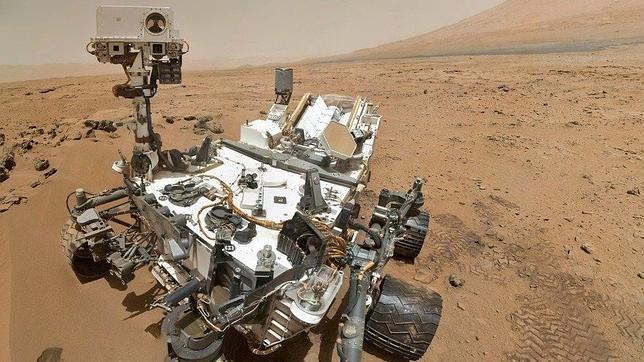
\includegraphics[scale=0.41]{imag/curiosity_marte.jpg}}\hspace{10mm}
	\subfloat[Teleoperación médica]{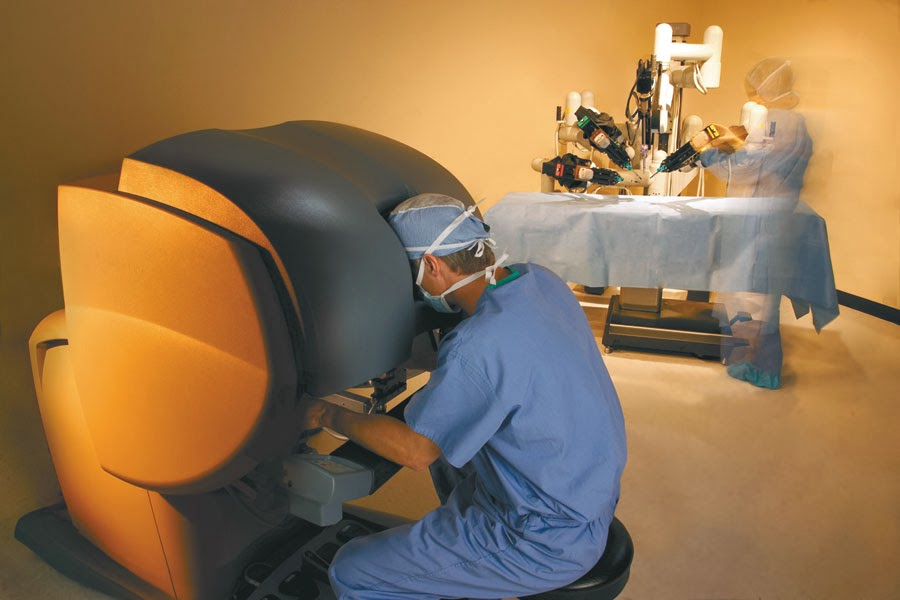
\includegraphics[scale=0.2]{imag/teleoperacion.jpg}}
	\caption{Ejemplos de robots}
	\label{FIG:1_robotica}
\end{figure}

\subsection{Aplicaciones actuales}\label{SEC:Aplic_actual}

Hoy en día, las aplicaciones de los robots son muy diversas. Fuera y dentro de nuestro planeta, los robots permiten ver sitios en los que el hombre no puede llegar directamente o en los que el hábitat es hostil como el Global Explorer ROV, que se ha sumergido en diferentes océanos para obtener imágenes nunca antes vistas por el hombre.

\subsubsection{Sector industrial}

Es uno de los sectores que compra más  robots y se encuentra en constante crecimiento. China pasó en 2013 a los E.E.U.U. en densidad de robots por trabajador y el número de ventas de robots industriales en el mundo aumentó un 16\%  en 2016 por cuarto año consecutivo (Figura \ref{FIG:_robotSales}\footnote{Datos obtenidos de International Federation of Robotics http://www.ifr.org/}\label{FN:IFR}). 

\begin{figure}[hbtp]
	\centering
	\subfloat{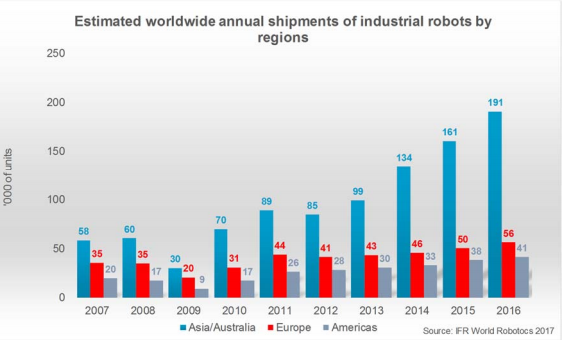
\includegraphics[scale=0.75]{imag/robotSales.png}}
	\caption{Ventas anuales estimadas de robots industriales por regiones}
	\label{FIG:_robotSales}
\end{figure}

Dentro de las aplicaciones industriales de robots encontramos:

\begin{itemize}
	\item Operaciones de manipulación: Usan pinzas, colaboran con otros robots y/u operarios y desplazan objetos. Este uso es uno de los más extendidos en empresas. Por ejemplo en el montaje de coches, ayudando a operarios a desplazar objetos pesados como las puertas.
	\item Soldadores. Se encargan de las tareas de soldadura de componentes. La compañía Asus ha creado un método de producción automático para sus tarjetas gráficas. En concreto, este proceso de soldadura mejora la calidad del producto y permite reducir el tamaño de sus tarjetas notablemente.\footnote{ASUS Auto-Extreme Technology: \url{https://www.youtube.com/watch?v=zVDEcu6-G3s}}
	\item Montaje. Las cadenas de montaje se vuelven más rápidas y eficientes. En las plantas de procesadores Intel, el proceso de montaje es uno de los más avanzados del mundo y se utilizan salas en las que el aire no es respirable para personas y garantizan una densidad de partículas externas muy baja, muy importante para la pureza de los procesadores.
\end{itemize}

\subsubsection{Aplicaciones de servicios}

El acercamiento de los robots a la población ha supuesto que su uso se encuentre en constante crecimiento y el número de aplicaciones es muy variado, desde recreación pasando por la grabación profesional para cine. A continuación se recogen algunas de las aplicaciones ilustrativas:

\begin{itemize}
	\item Limpieza doméstica: Incluye robots que limpian piscinas, hasta aspiradoras inteligentes. Este último caso es el de Roomba, de la compañía iRobot, que incorpora algoritmos de construcción de mapas, evasión de objetos o incluso detección de escaleras (para evitar posibles accidentes).
	
	\item Transporte de personas: Los mayores representante de este tipo de productos son Waymo, Tesla y Uber(Figura \ref{FIG:1_Aplicaciones}). En esta categoría se recogen sistemas de seguridad que controlan la distancia de seguridad respecto de otros vehículos, los sistemas de aparcamiento asistido o habilitar a personas con movilidad reducida o discapacitados para que puedan usar los automóviles. Para ejecutar estas tareas los vehículos están equipados con todo tipo de sensores que permiten la autolocalización, evitar accidentes y llegar al destino deseado. Algunas compañías como Uber y Tesla han sufrido recientemente accidentes mortales que pueden retrasar esta aplicación en el futuro.
	
	\item Ocio y entretenimiento: La utilización de drones con la capacidad de volar ha reducido considerablemente el coste de planos aéreos y simplificado el equipo necesario. Airdog (Figura \ref{FIG:1_Aplicaciones}) es un proyecto nacido de una campaña Kickstarter que permite el seguimiento de actividades deportivas o recreativas a gran velocidad, de forma totalmente autónoma, y la grabación de las mismas.
	
	\item Educación: La aplicación de robots para el uso didáctico se contempla como un recurso innovador, que aumenta el interés de los niños y sirve de apoyo para los maestros (Figura \ref{FIG:1_Aplicaciones}).
	
	\item Militar y seguridad: Para evitar la pérdida de bajas humanas, aumentar la capacidad de motorización y mejorar su potencia de combate. Los ejércitos están invirtiendo cada vez más en robots capaces de sustituir a soldados en el frente y como armas de defensa.
	
\end{itemize}

\begin{figure}[hbtp]
	\centering
	\subfloat[Tecnología Tesla autopilot]{\includegraphics[scale=0.21]{imag/tesla-autopilot.jpg}}\hspace{5mm}
	\subfloat[Secuencia de seguimiento de un Airdog]{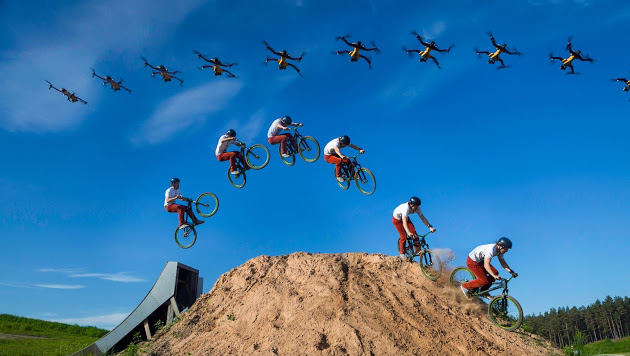
\includegraphics[scale=0.21]{imag/air_dog.jpg}}\hspace{5mm}
	\subfloat[Robot PEPPER en un aula como complemento educador]{\includegraphics[scale=0.4]{imag/pepper.jpeg}}\hspace{5mm}
	\caption{Aplicaciones en la actualidad}
	\label{FIG:1_Aplicaciones}
\end{figure}

\section{Software en robots}\label{SEC:Software en robots}

El software que se encuentra en los robots es el encargado de dotar de un comportamiento inteligente a los mismos. 

Puede estar formado por sistemas complejos, aplicaciones e infraestructuras que son las responsables de las acciones del robot. Las fases del desarrollo del software robótico son muy similares a las del desarrollo de software en otros ámbitos, donde a partir de ciertos requisitos, se modela un diseño que será implementado. Durante años este desarrollo se ha centrado en resolver los problemas con soluciones \textquoteleft ad-hoc\textquoteright, es decir, creando un diseño para un robot con sensores y actuadores específicos. Esto requería que se realizase una implementación nueva por cada robot diferente, a pesar de que las características fueran similares. En la actualidad, gracias a la existencia de diferentes plataformas de desarrollo para robots es posible diseñar e implementar soluciones que puedan aplicarse de forma eficiente y genérica. Esto permite reutilizar herramientas, aplicaciones y algoritmos creados con antelación y reducir los costes durante la fase de desarrollo del software.


\subsection{Simulación}\label{SEC:Simulacion}

Una parte muy importante a la hora de diseñar el comportamiento de un robot es la simulación ya que permite probar algoritmos sin necesidad de utilizar uno real. Esto nos aporta información muy valiosa y facilita la familiarización con posibles situaciones que no hayamos pensado con suficiente antelación, además de prevenir accidentes como por ejemplo cualquier daño físico al robot o herir a las personas cercanas. Una vez se alcance un comportamiento que cumpla nuestras expectativas, se procederá a ponerlo a prueba en el robot real teniendo en cuenta que muy probablemente aparecerán anomalías en el comportamiento no detectadas durante la fase de simulación. Esta diferencia en el comportamiento depende de la precisión con la que se ha caracterizado el modelo del robot y el escenario virtual con el que interacciona. Esto se debe a siempre existe un grado de aproximación entre la virtualización y el mundo real. Muchos simuladores incluyen la adición de funciones de ruido en sensores y actuadores para alcanzar un comportamiento mucho más próximo al real.

Un ejemplo es Gazebo\footnote{Página web oficial de Gazebo : \url{http://gazebosim.org/}}, un proyecto de software libre que incluye multitud de modelos y motores de física virtualizada. Ofrece una interfaz gráfica y control sobre los objetos y el mundo generado, además de la creación y modificación de actuadores y sensores personalizados. Por ejemplo, se pueden crear vehículos con diferentes sensores o casas con las que interactuar.

\begin{figure}[hbtp]
	\centering
	{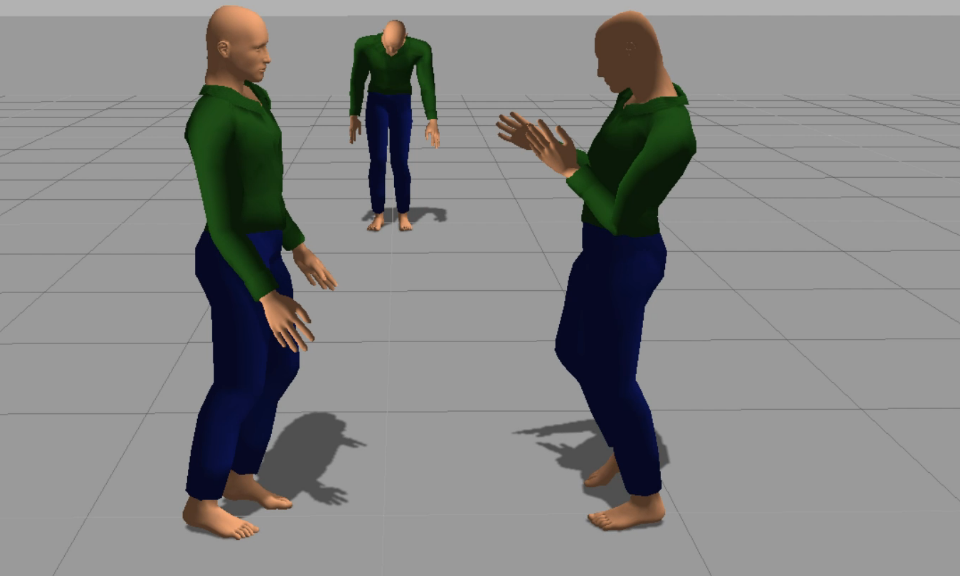
\includegraphics[scale=0.3]{imag/gazebo2.png}}\hspace{10mm}
	%\subfloat[Personas en Gazebo]{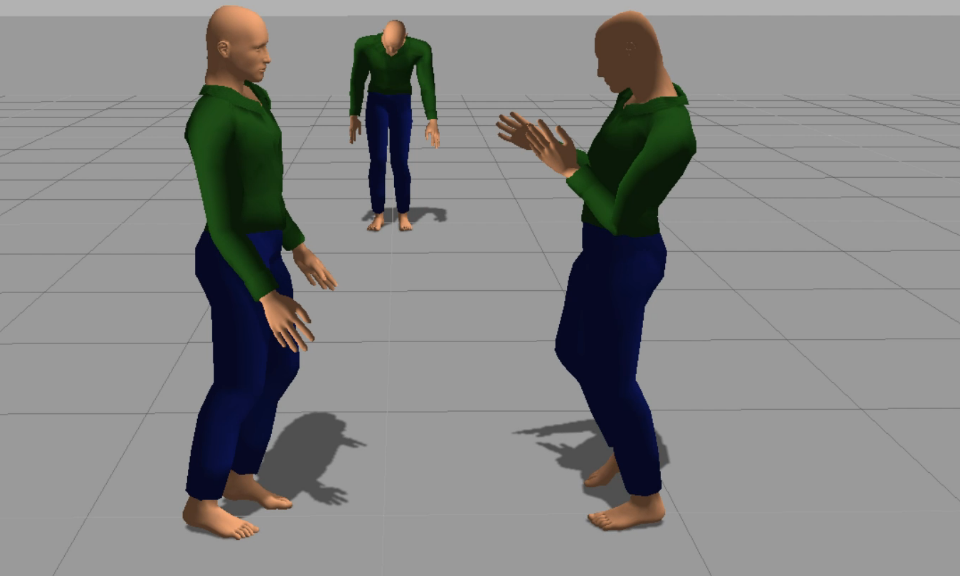
\includegraphics[scale=0.26]{imag/gazebo2.png}}
	\caption{Personas simuladas en Gazebo}
	
	\label{FIG:6_simulacion}
\end{figure}


\section{Visión artificial en robots}\label{SEC:Vision artificial en robots}

La visión artificial, también conocida como visión por computador, es un subcampo de la inteligencia artificial en la que mediante el procesado y análisis de imágenes se trata de extraer información en un computador aplicando transformaciones y algoritmos basados en diferentes disciplinas como por ejemplo la estadística, geometría o \textit{machine learning}.

La visión para los robots, al igual que para las personas, es una gran fuente de información del entorno. Las personas utilizamos el espectro visible de la luz, que se corresponde con lo que llamamos colores. Además, percibimos el mundo que nos rodea como un mundo en tres dimensiones debido a que tenemos dos ojos. Esto nos permite obtener propiedades del entorno y poder  desplazarnos en él sin preocupaciones. Los robots utilizan sensores de visión de todo tipo, capaces de ver en la oscuridad o distinguir diferentes temperaturas. Además, en los últimos años, los sensores de visión han disminuido en precio y su utilización se ha visto incrementada notablemente en el mundo de la robótica, pasando a ser un equipamiento muy común en los robots. En este TFG, utilizaremos dos cámaras para obtener las imágenes que una vez procesadas aportarán la información necesaria para dotar de un comportamiento autónomo al drone.

Existen diferentes bibliotecas que recogen algoritmos y herramientas para simplificar la visión artificial. Cabe destacar \textit{OpenCV}, como la biblioteca  de código libre más extendida a la hora de realizar visión artificial en robots. Esta biblioteca, de la que hablaremos más adelante en detalle \ref{sec:opencvs}, ha facilitado la introducción y la aplicación de técnicas avanzadas de visión artificial para realizar el análisis y procesado de imágenes. Además, podemos encontrar en Internet numerosos ejemplos y tutoriales en los que se muestran las capacidades y aplicaciones de esta biblioteca.

\textit{DeepLearning} (aprendizaje jerárquico), es una familia de técnicas de procesamiento de imágenes basada en \textit{machine learning}. En los últimos años la aplicación de estas técnicas ha dado muy buenos resultados, especialmente dotando de una mayor robustez en comparación a los algoritmos más tradicionales creados para una tarea en específico. 

Actualmente, las aplicaciones de visión artificial en robots son muy variadas, desde seguridad, como sistemas de detección de movimiento, pasando por el entretenimiento, como el sensor Kinect, hasta la accesibilidad para dotar de autonomía a personas que lo necesitan. Para esto se utilizan las siguientes técnicas: 

\begin{itemize}
	\item Construcción de mapas: Es una de las primeras aplicaciones a través de visión y permite a los robots la creación de mapas a través de la detección de bordes, formas o profundidad. Ésta información sirve también para poder navegar sobre sitios desconocidos o previamente han sido convertidos a un mapa \ref{FIG:5_vision}.
	\item Autolocalización: Permite extraer información a un robot sobre la posición relativa respecto al resto del mundo que lo rodea, mediante el reconocimiento de patrones o balizas. Una técnica es el SLAM \ref{FIG:5_vision} (\textit{Simultaneous Localization and Mapping}), que permite la autolocalización al mismo tiempo que se realiza un mapa del entorno. 
	\item Detección e identificación de objetos: El reconocimiento o identificación de objetos\ref{FIG:5_vision} se consigue a partir de la extracción de características únicas de cualquier objeto o persona que podemos encontrar en una imagen. La aplicación de DeepLearning está llevando cada vez más lejos los límites de este reconocimiento, dando lugar a un reconocimiento de objetos mucho más robusto, superando al ser humano en determinadas condiciones.
	\item Navegación y control visual: Permite la navegación autónoma o asistida de robots. Actualmente, se emplea en entornos industriales o el sector de la automoción para el desplazamiento de objetos o personas.
\end{itemize}

\begin{figure}[hbtp]
	\centering
	\subfloat[Reconocimiento de objetos en imagen]{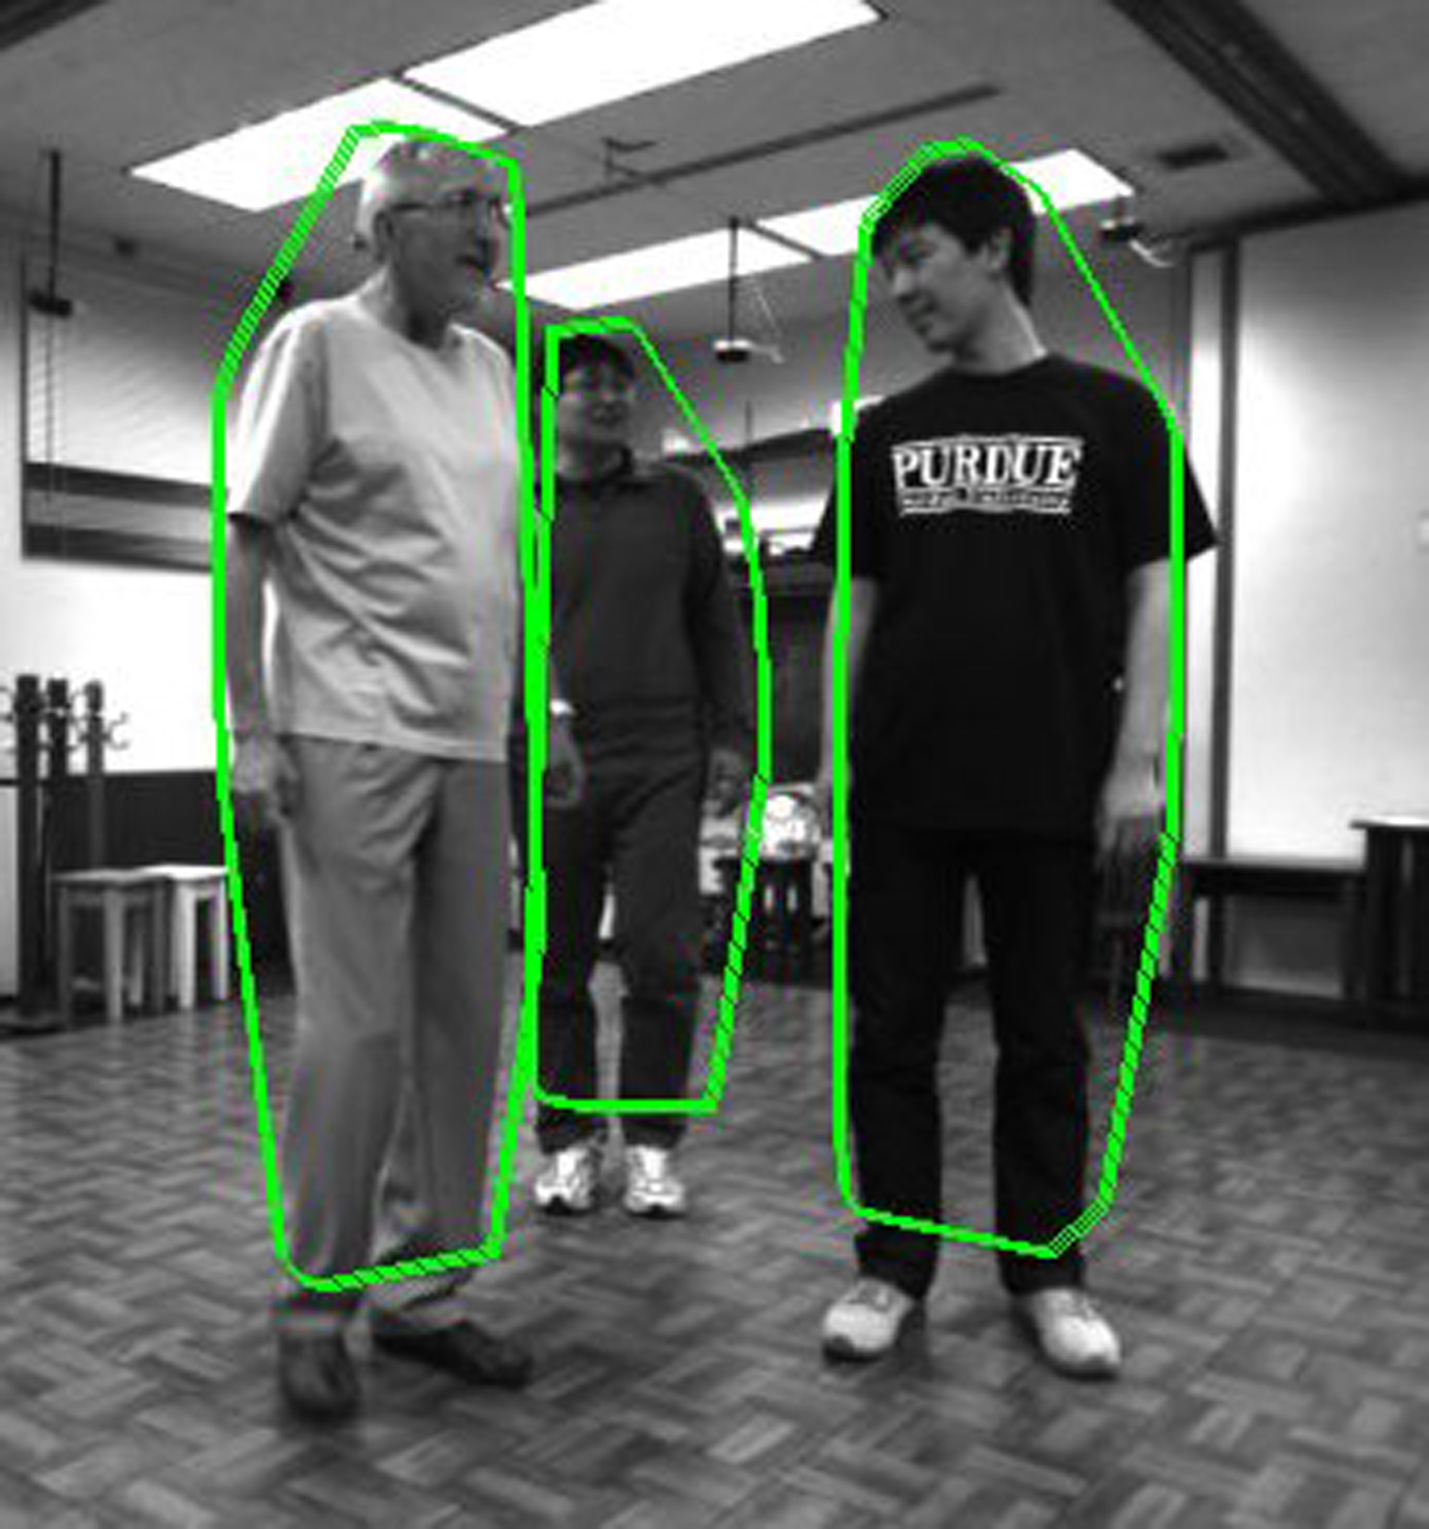
\includegraphics[scale=0.4]{imag/robotic_vision1.jpg}}\hspace{10mm}
	\subfloat[Reconstrucción de mapas con técnicas SLAM]{\includegraphics[scale=0.255]{imag/mapaimagen.jpg}}
	\caption{Visión artificial en robots}
	
	\label{FIG:5_vision}
\end{figure}


\section{Robótica Aérea}\label{SEC:Robotica Aerea}

Es una de las ramas de la robótica de mayor auge actualmente y sus aplicaciones son cada vez más extendidas. Pertenecen a este área los \textit{Unmanned Aircraft Vehicle}(UAV), en español \textit{Vehículo Aéreo No Tripulado}(VANT), o también conocidos como \textit{drones}. Se trata de un vehículo capaz de volar, que puede o no recibir órdenes del exterior. Incluyen multitud de diferentes sensores para mantenerse en vuelo, aterrizar o despegar.

Históricamente, el origen de los UAV ha sido en aplicaciones militares, como en otras áreas de investigación. Una vez ha sido suficientemente desarrollado comienzan las aplicaciones civiles y su aplicación comercial e industrial.
Durante la primera y la segunda guerra mundial se utilizaron drones para la obtención de mapas sin poner en peligro al piloto. Más tarde, en 1995 se utilizaron en Bosnia para tareas de vigilancia o análisis de daños, siendo especialmente importante para el reconocimiento nocturno. El modelo se llamaba \textit{Predator} \ref{FIG:8_historia2}.

\begin{figure}[hbtp]
	\centering
	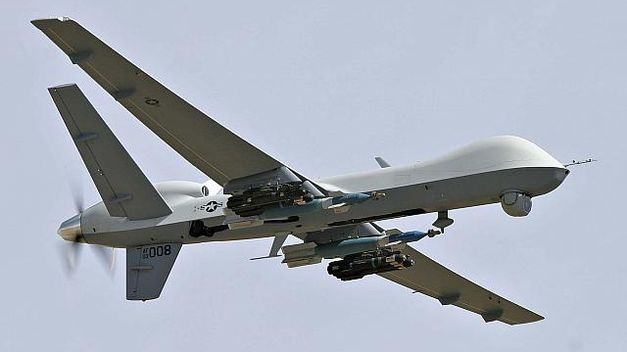
\includegraphics[scale=0.25]{imag/predator.jpg}
	\caption{UAV Predator.}
	
	\label{FIG:8_historia2}
\end{figure}

\subsection{Aplicaciones actuales}

Actualmente, gracias al avance de la estabilización electrónica, los UAV han alcanzado tamaños mucho más reducidos, como el \textit{Hummingbird}\footnote{Más información en: \url{http://www.avinc.com/nano}} o colibrí en español, de \textit{DARPA}. Además son mucho más ágiles y mecánicamente simples. Han aparecido numerosos usos comerciales y civiles, aunque no desaparece el interés militar. Compañías como \textit{Amazon} \ref{FIG:9_historia2}, están trabajando en proyectos para conseguir crear un sistema de envío de compra a domicilio utilizando \textit{drones}, en concreto \textit{cuadricópteros}.
 
Intel está diseñando comportamientos basados en grupos masivos, creando formaciones en el aire y dotando capacidad de pensamiento en grupo a los drones.
 
Otro de los usos es la exploración aérea, que incluye la inspección de embalses, líneas de alta tensión, campos agrícolas y la vigilancia. Este último caso es el de Alemania, que utiliza drones aéreos para evitar el ataque de grafiteros a vagones de tren\footnote{Alemania pone a prueba drones contra los grafitis: \url{http://www.bbc.com/mundo/noticias/2013/05/130528_tecnologia_drones_graffiti_alemania_aa}}.

Uno de los campeonatos más recientes de programación para UAV es el \textit{Mohamed Bin Zayed International Robotics Challenge}(MBZIRC)\footnote{Página Web oficial del campeonato: \url{http://www.mbzirc.com/}}. Con una recompensa de 5 millones de dólares, una de las pruebas consiste en localizar, seguir y aterrizar, coincidiendo con los objetivos principales de este Trabajo Fin de Grado.

\begin{figure}[hbtp]
	\centering
	\subfloat[Modelo utilizado por Amazon Air Prime.]{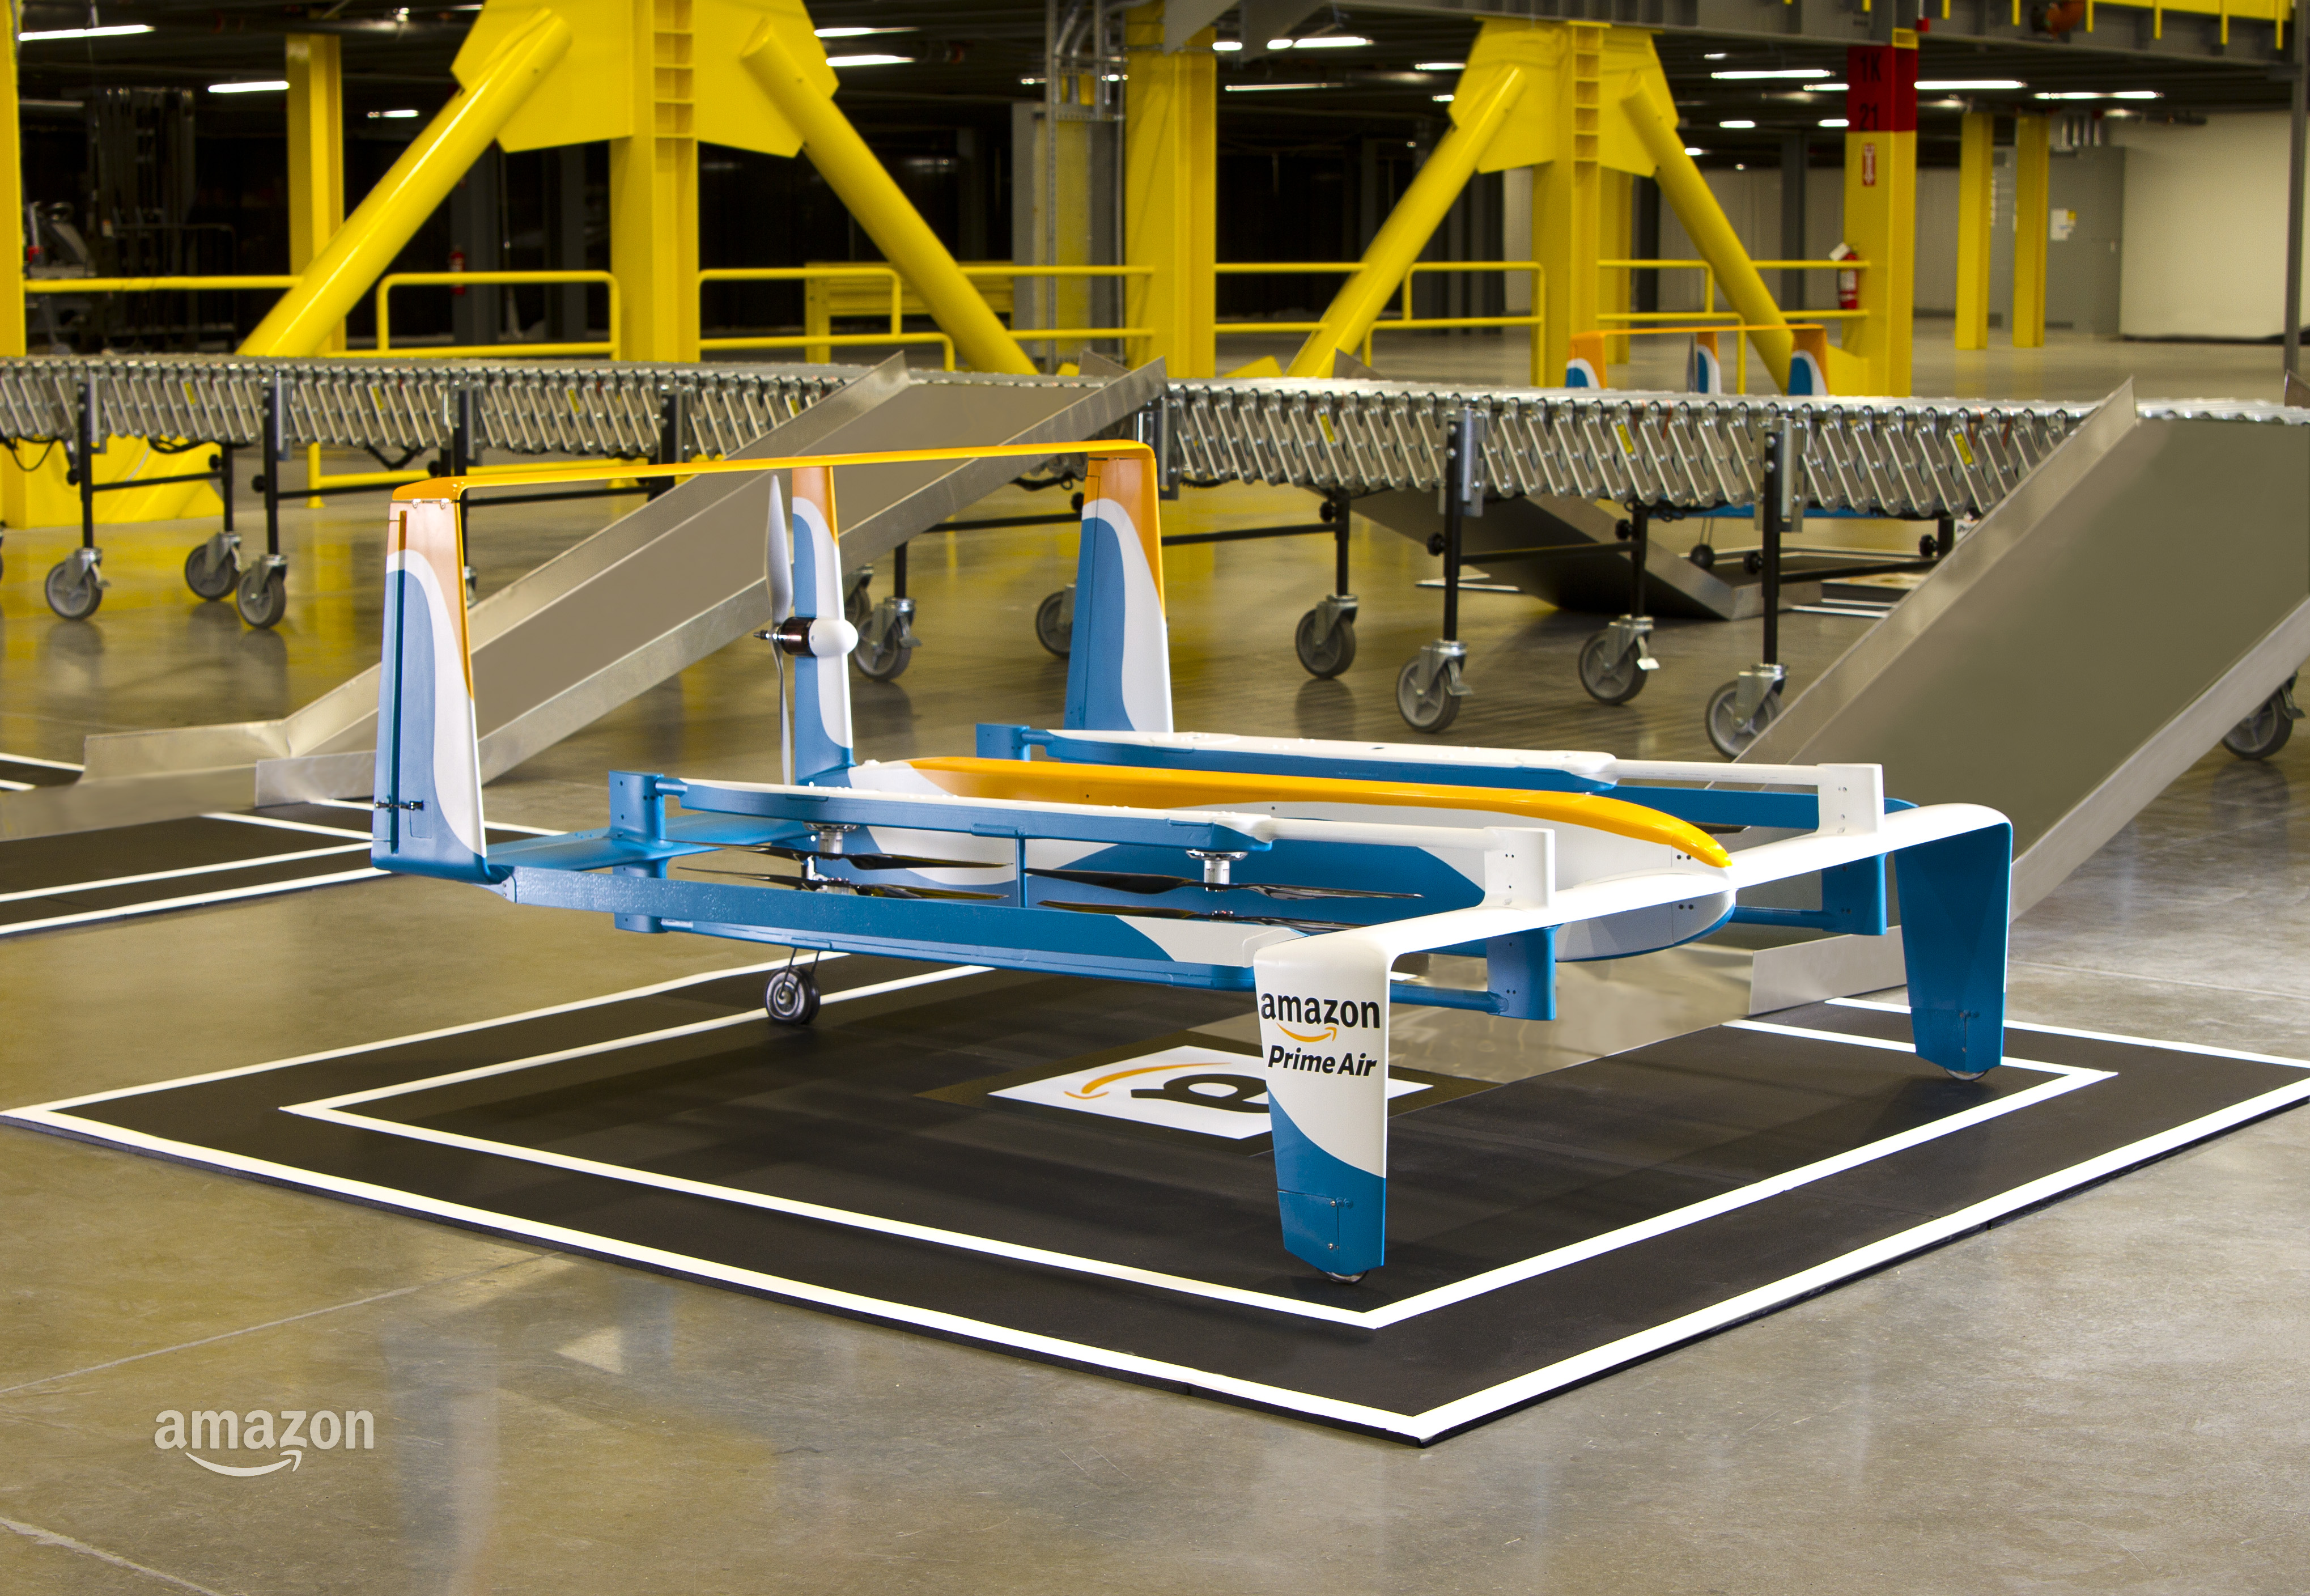
\includegraphics[scale=0.14]{imag/prime-air_03.jpg}}\hspace{5mm}
	\subfloat[Actuación de drones masivos durante la de apertura de los J.J.O.O de Invierno 2018]{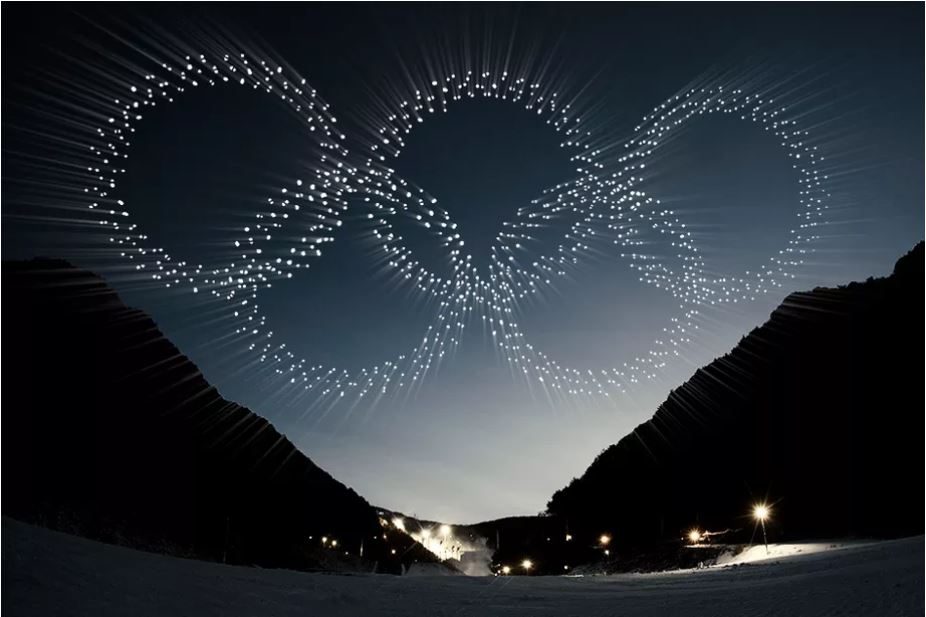
\includegraphics[scale=0.26]{imag/inteldrones.jpg}}
	\caption{Ejemplos de UAV civiles}	
	\label{FIG:9_historia2}
\end{figure}

\subsubsection{Cuadricópteros}

Existen diferentes tipos de drones en función del diseño y los componentes que los forman. Algunos son similares a los aviones, con alas y el mismo método de despegue y aterrizaje. Están pensados para largos períodos de tiempo y altas velocidades. Otros buscan una excepcional maniobrabilidad y estabilidad aérea. En este caso utilizan rotores, al igual que los helicópteros. A este grupo pertenecen los cuadricópteros. Se caracterizan por ser un helicóptero multi-rotor de cuatro brazos en forma de cruz. Los rotores se encuentran en el extremo de cada brazo. 

Cuando los motores giran las hélices situadas en ellos generan un fuerza de empuje vertical llamada \textit{sustentación}. Ésta es perpendicular al movimiento de la hélice y depende de la velocidad a la que gira. La suma de cada fuerza en cada rotor produce una resultante. Los diferentes movimientos que puede describir el cuadricóptero se encuentran recogidos en la Figura\ref{FIG:10_historia2}. El color rojo indica que una potencia mayor ha sido aplicada, mientras que el verde, representa una potencia menor. Para evitar un fenómeno que en los helicópteros produce vueltas sobre sí mismo, la disposición de los motores sigue una forma de cruz, en la que cada par opuesto gira en el mismo sentido. Uno en el sentido de las agujas del reloj y el otro anti-horario.

Para que sea posible el despegue (Figura\ref{FIG:10_historia2},e), esta resultante ha de ser superior al peso del UAV. Si es igual, el drone queda cernido en una altitud fija (\textit{hovering}). Para aterrizar sería necesario una resultante menor que el peso del objeto (Figura\ref{FIG:10_historia2},f).

El giro conocido como \textit{yaw} (Figura\ref{FIG:10_historia2},g y h) o \textit{guiñada}, es el giro del plano horizontal al drone. Para girar a la derecha se transmite más potencia al par de rotores que giran en sentido anti-horario. Si la potencia fuera superior en el otro par opuesto, giraría hacia la izquierda sobre sí mismo.

En el supuesto de que sólo uno de los motores aplicase más potencia que los demás, por ejemplo el delantero, el cuadricóptero se desplazaría hacia atrás, inclinando la parte trasera del vehículo hacia arriba. Esto se correspondería con el movimiento llamado \textit{pitch} (Figura\ref{FIG:10_historia2},a y b) o \textit{cabeceo}.

Por último, si aumentamos la potencia en uno de los motores laterales, por ejemplo la derecha, el vehículo se inclinará y trasladará hacia la izquierda, provocando un movimiento conocido como \textit{roll} (Figura\ref{FIG:10_historia2},c y d) o \textit{alabeo}. 

\begin{figure}[hbtp]
	\centering
	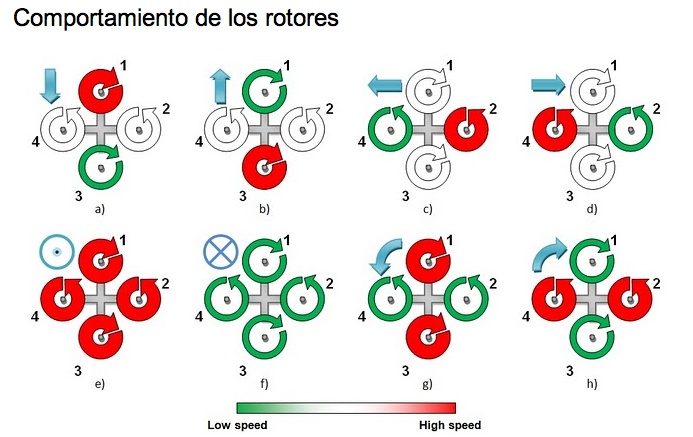
\includegraphics[scale=0.6]{imag/rotores.png}
	\caption{Relación entre la potencia de los rotores y el movimiento de un cuadricóptero}
	\label{FIG:10_historia2}
\end{figure}
Los cuadricópteros pueden tener numerosos sensores a bordo desde acelerómetros, giroscopios, magnetómetros, ultrasonidos, incluso cámaras con resoluciones de hasta 4K. Todo ello se utiliza en combinación para conseguir una mayor estabilización durante el vuelo. Dentro de los actuadores encontramos los cuatro rotores pero también se pueden añadir pinzas para cargar objetos o, en caso de uso militar, armas y sus respectivos gatillos.

Algunos de los fabricantes de cuadricópteros más relevantes actualmente son:

\begin{itemize}
	\item Parrot: Con modelos como el Ar.Drone que acercaron a un gran público el uso de los drones. Actualmente el modelo Bebop 2 \footnote{https://www.parrot.com/us/drones/parrot-bebop-2} ofrece una cámara frontal con resolución \textit{FullHD}, soporte para controles en dispositivos móviles e integración con gafas de realidad virtual para teleoperar el drone.
	\item  Erle: El Erle-Copter \footnote{http://erlerobotics.com/blog/Erle-Copter/} soportado oficialmente por Ubuntu y por el \textit{middleware} robótico ROS (Robot Operating System), facilitando el desarrollo de software en este drone. Está pensado para la instalación de módulos nuevos y así adaptarse a diferentes situaciones.
	\item  DJI: Una de las compañías que más drones vende anualmente, cargados de todo tipo de sensores, cámaras con las últimas tecnologías de estabilización y algoritmos inteligentes de navegación. Su modelo Inspire 2 \footnote{https://www.DJI.com/es/inspire-2?site=brandsite\&from=nav} es muy utilizado en el mundo audiovisual y el cine.
\end{itemize}

\subsubsection{Robótica Aérea en el proyecto JdeRobot}

El proyecto JdeRobot de software libre para robótica lleva años desarrollando proyectos relacionados con la navegación, visión, autolocalización y virtualización de entornos con robots. Gracias a la popularización y a la reducción en coste de los drones se comenzó en el año 2013 una nueva línea de investigación en JdeRobot sobre los UAV. Los primeros proyectos han creado las bases sobre las que seguir investigando y han proporcionado la infraestructura necesaria. Sirven como base antecedentes directos y contexto cercano de este TFG.

Entre estos proyectos se encuentra el Trabajo de Fin de Grado(TFG) \textit{Navegación visual en robots aéreos} de Alberto Martín \cite{AlbertoMartin}. Sus aportaciones fueron la de un driver llamado \textit{ardrone\_server}, que crea una interfaz capaz de comunicarse con el \textit{AR.Drone} de la compañía Parrot. El mismo trabajo incluye una herramienta llamada \textit{uav\_viewer} \ref{FIG:11_uav_viewer}, cuya función es obtener la información de los sensores y teleoperar los actuadores de dicho UAV. Por último, aportó un componente de visión y navegación llamado \textit{object\_tracking} que utiliza filtros de colores para el seguimiento de objetos a través de las imágenes recibidas por la cámara frontal y ventral del drone. El drone es  capaz de un seguimiento autónomo de objetos, tanto en el suelo como en 3D.

\begin{figure}[hbtp]
	\centering
	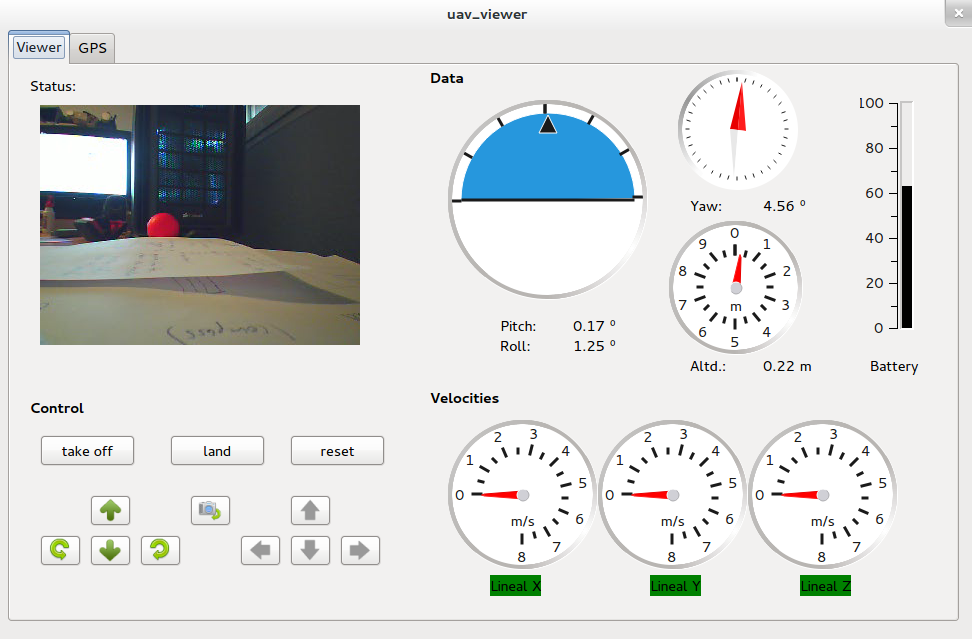
\includegraphics[scale=0.35]{imag/uav_viewer.png}
	\caption{Ejemplo de interfaz de usuario del componentes Uav\_viewer}	
	\label{FIG:11_uav_viewer}
\end{figure}

Daniel Yagüe en su Proyecto Fin de Carrera \textit{Cuadricóptero AR.Drone en Gazebo y JdeRobot} \cite{DanielYague}, desarrolló un modelo y un driver en el simulador Gazebo del mismo AR.drone \ref{FIG:ardronegazebo} que utilizó Alberto Martín. Esto permite tanto la simulación de los datos sensoriales como de la virtualización realista de un comportamiento cercano a dicho drone. Adicionalmente, programó diferentes aplicaciones de navegación autónomas como el seguimiento de balizas por posición, de carretera o de otro cuadricóptero.

\begin{figure}[hbtp]
	\centering
	\subfloat[Modelo de Ar.Drone en Gazebo.]{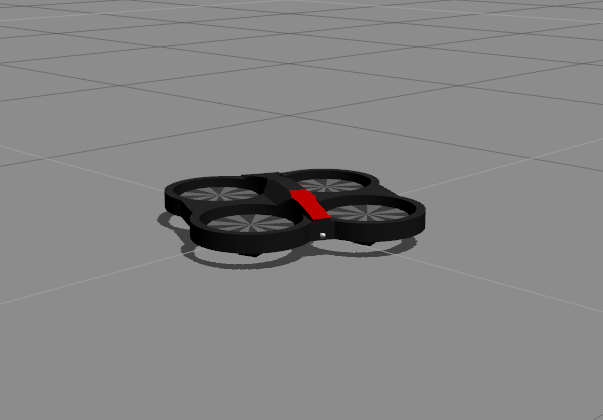
\includegraphics[scale=0.311]{imag/ArDrone_model.png}}\hspace{5mm}
	\subfloat[Modelo Ar.Drone teleoperado en Gazebo]{\includegraphics[scale=0.19]{imag/danielyaguedrone.jpg}}
	\caption{Ejemplos de ArDrone simulado en Gazebo}	
	\label{FIG:ardronegazebo}
\end{figure}

Por otro lado Alberto López-Cerón, con su TFM \textit{Autolocalización visual robusta basada en marcadores} \cite{AlbertoLopez}, creó un algoritmo capaz de estimar la posición de la cámara a partir de la detección de marcadores o balizas. Manuel Zafra siguió desarrollando la idea de Alberto López-Cerón en \textit{Seguimiento de rutas 3D por un drone con autolocalización visual con balizas} \cite{ManuelZafra}. Diseñó un algoritmo de navegación en interiores basado en autolocalización mediante la visión artificial en simulador \ref{FIG:ejemploautolocalizacion}.

\begin{figure}[hbtp]
	\centering
	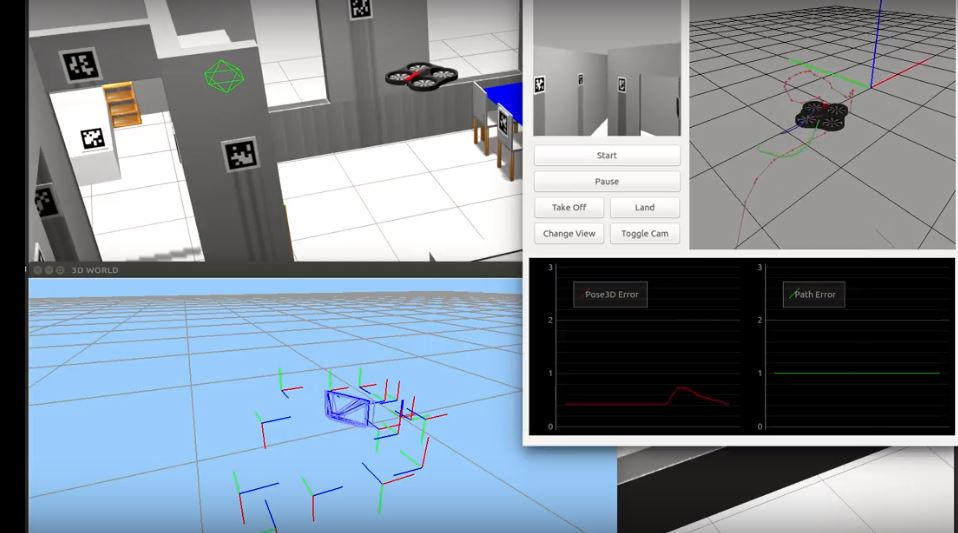
\includegraphics[scale=0.55]{imag/ejemploautolocalizacion.jpg}
	\caption{Ejemplo de algoritmo de navegación basado en autolocalización en Gazebo.}	
	\label{FIG:ejemploautolocalizacion}
\end{figure}


Jorge Vela se centró en el \textit{Despegue, navegación y aterrizaje visuales de un drone usando JdeRobot} \cite{JorgeVela}. Sentó las bases para el despegue y aterrizaje controlado utilizando visión artificial en un drone real \ref{FIG:despgueyaterrizaje}

\begin{figure}[hbtp]
	\centering
	\subfloat[Algoritmo de despegue y aterrizaje encontrando la baliza visual en Gazabo.]{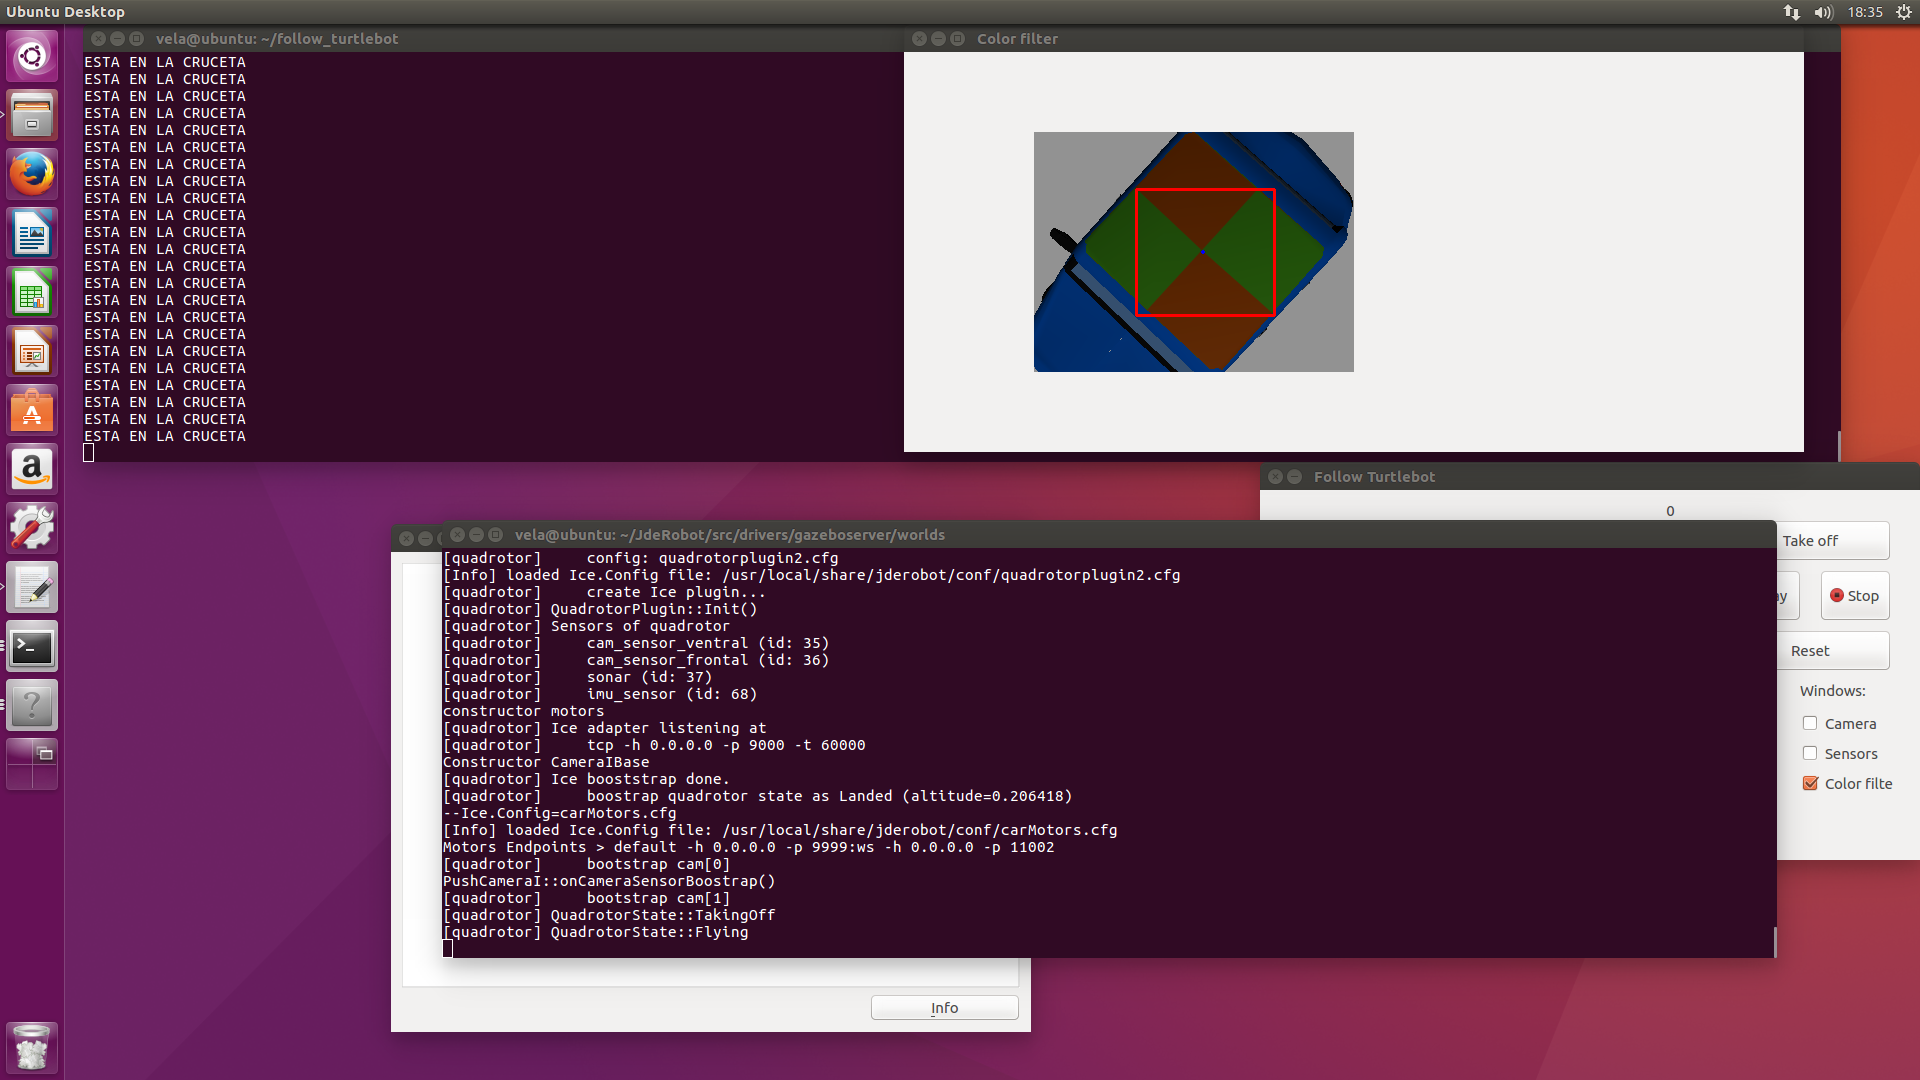
\includegraphics[scale=0.12]{imag/L_CenteringCar.png}}\hspace{2mm}
	\subfloat[Ar.Drone en vuelo sobre baliza visual.]{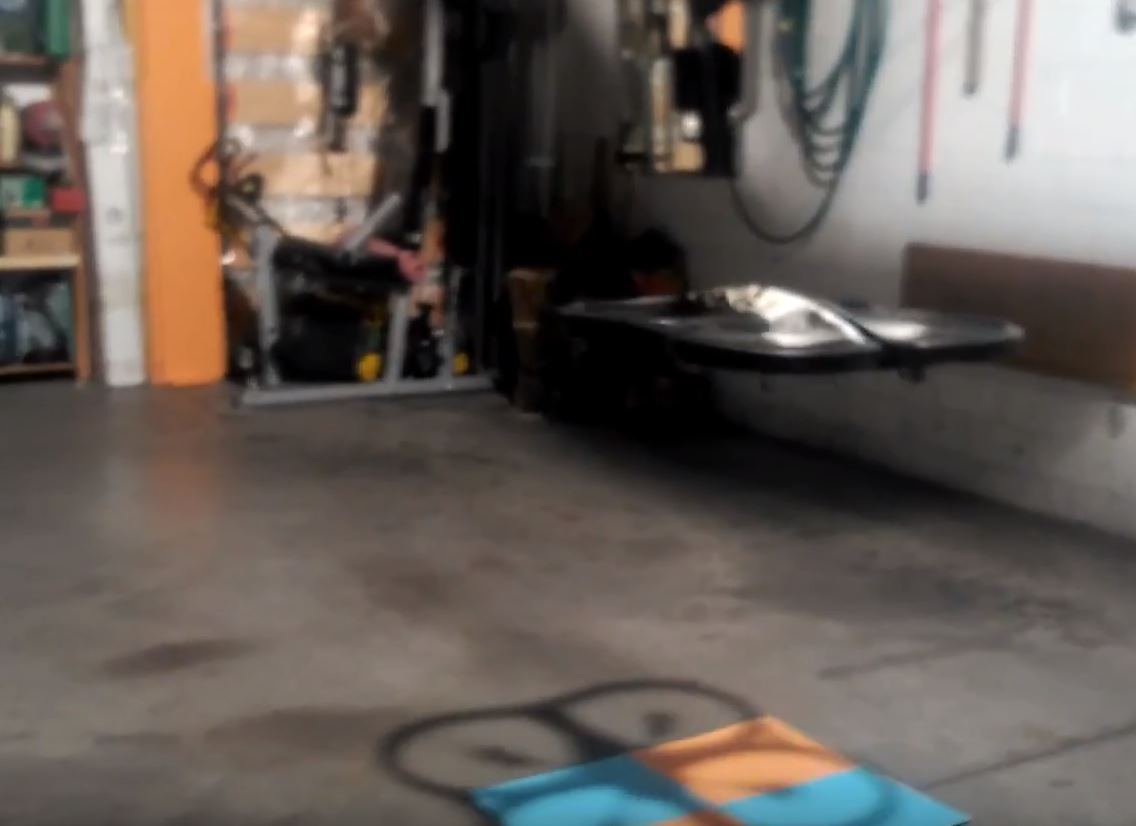
\includegraphics[scale=0.22]{imag/aterrizajereal.jpg}}
	\caption{Ejemplos de aterrizaje y despegue en Gazebo y el drone real.}	
	\label{FIG:despgueyaterrizaje}
\end{figure}

Jesús Saiz, en su TFG \textit{Programación de un drone para seguimiento autónomo de trayectorias en 3D} \cite{JesusSaiz}, integró el algoritmo de despegue y aterrizaje controlados y la autolocalización visual basada en balizas para crear un autómata de estados finito que navega de forma autónoma a través de rutas predefinidas en el simulador Gazebo. 

\begin{figure}[hbtp]
	\centering
	\includegraphics[scale=0.25]{imag/SlamMarkersJesus.jpg}
	\caption{Ejemplo de navegación a través del seguimiento de rutas.}	
	\label{FIG:ejemplonavegacion}
\end{figure}



Siguiendo con las bases aportadas por todos estos proyectos, en este TFG se programará el comportamiento autónomo de despegue controlado y aterrizaje de un drone sobre una baliza visual y la navegación a partir de la autolocalización. Se utilizará un drone real, empleando la infraestructura existente en JdeRobot para estos cuadricópteros. Con ello se pretende unificar los avances anteriores en un drone real y dejó la puerta abierta a nuevos comportamientos más sofisticados.


En el próximo capítulo se explicarán los objetivos y la metodología propuesta para resolverlos. En el tercer capítulo se expondrán con profundidad la infraestructura y herramientas  utilizadas. En el cuarto, se describirá el desarrollo de todos los componentes que forman este proyecto. En quinto lugar, se detallarán los distintos experimentos para validar experimentalmente la solución programada. Para terminar, unas conclusiones aportarán un visión global del conjunto y los conocimientos extraídos.

